\subsection{Excercise APIDIagramAMRentalManagementV1.0}
TODO Add introduction
\subsubsection*{Derivation of the API Diagram}
An API diagram models the relevant entities depending on the type of API, in this case, \hfill \linebreak \texttt{RentalManagementV1.0} is an application microservice.
In an AM API diagram, relations between the application entities and the entities from other API diagrams occur.
A copy of the API diagram can be found on \url{https://gitlab.kit.edu/kit/cm/teaching/carrentalapp/0.doccarrentalappv1/-/blob/main/figures/ad_am-rental_management_v1.0.png?ref_type=heads} is shown in \autoref*{fig:ad_am-rental_management_v1.0}.

% Which artifacts are used to derive the API diagram
Since \texttt{RentalManagementV1.0} interacts with the \texttt{DM-CarV1.0} domain microservice, the DM API diagram is one artifact used to derive the AM API diagram.
Using the DM API diagram, the application entity \texttt{Car} is modeled.
Next, the entity diagram of \texttt{CarRental} is used to derive the application entities, their functions and their relations.
This entity diagram is shown in \autoref{fig:extendedEntityDiagram}
Yet, not all functions can be derived by \texttt{CarRental} alone.
The Use Cases of \texttt{CarRental} are used to derive functions too.
Advancing in this thesis, these Use Cases are also used to derive the CLI commands for \texttt{CarRentalCLI}.
Despite not all commands being implemented in this microservice, the functions for renting and canceling a rental are implemented, being specified by the Use Cases and the according CLI commands.

% How are the entities and methods established
The application entities \texttt{Customer} and \texttt{Rental} are derived from the entity diagram \autoref{fig:extendedEntityDiagram}.
Both entities keep the same attributes and relations as in the entity diagram.
The entity \texttt{Car} is derived from the DM API diagram, yet the relation between \texttt{Car} and \texttt{Rental} stays the same as in the entity diagram.
Last, the collection \texttt{Rentals} is newly created.
It contains a list of rentals and the \texttt{listAvailableCars} function returning a list of available cars.
Therefore, it is derived from the general structure and functionality of \texttt{DM-CarV1.0}'s \texttt{Cars} collection.

\begin{figure}
    \centering
    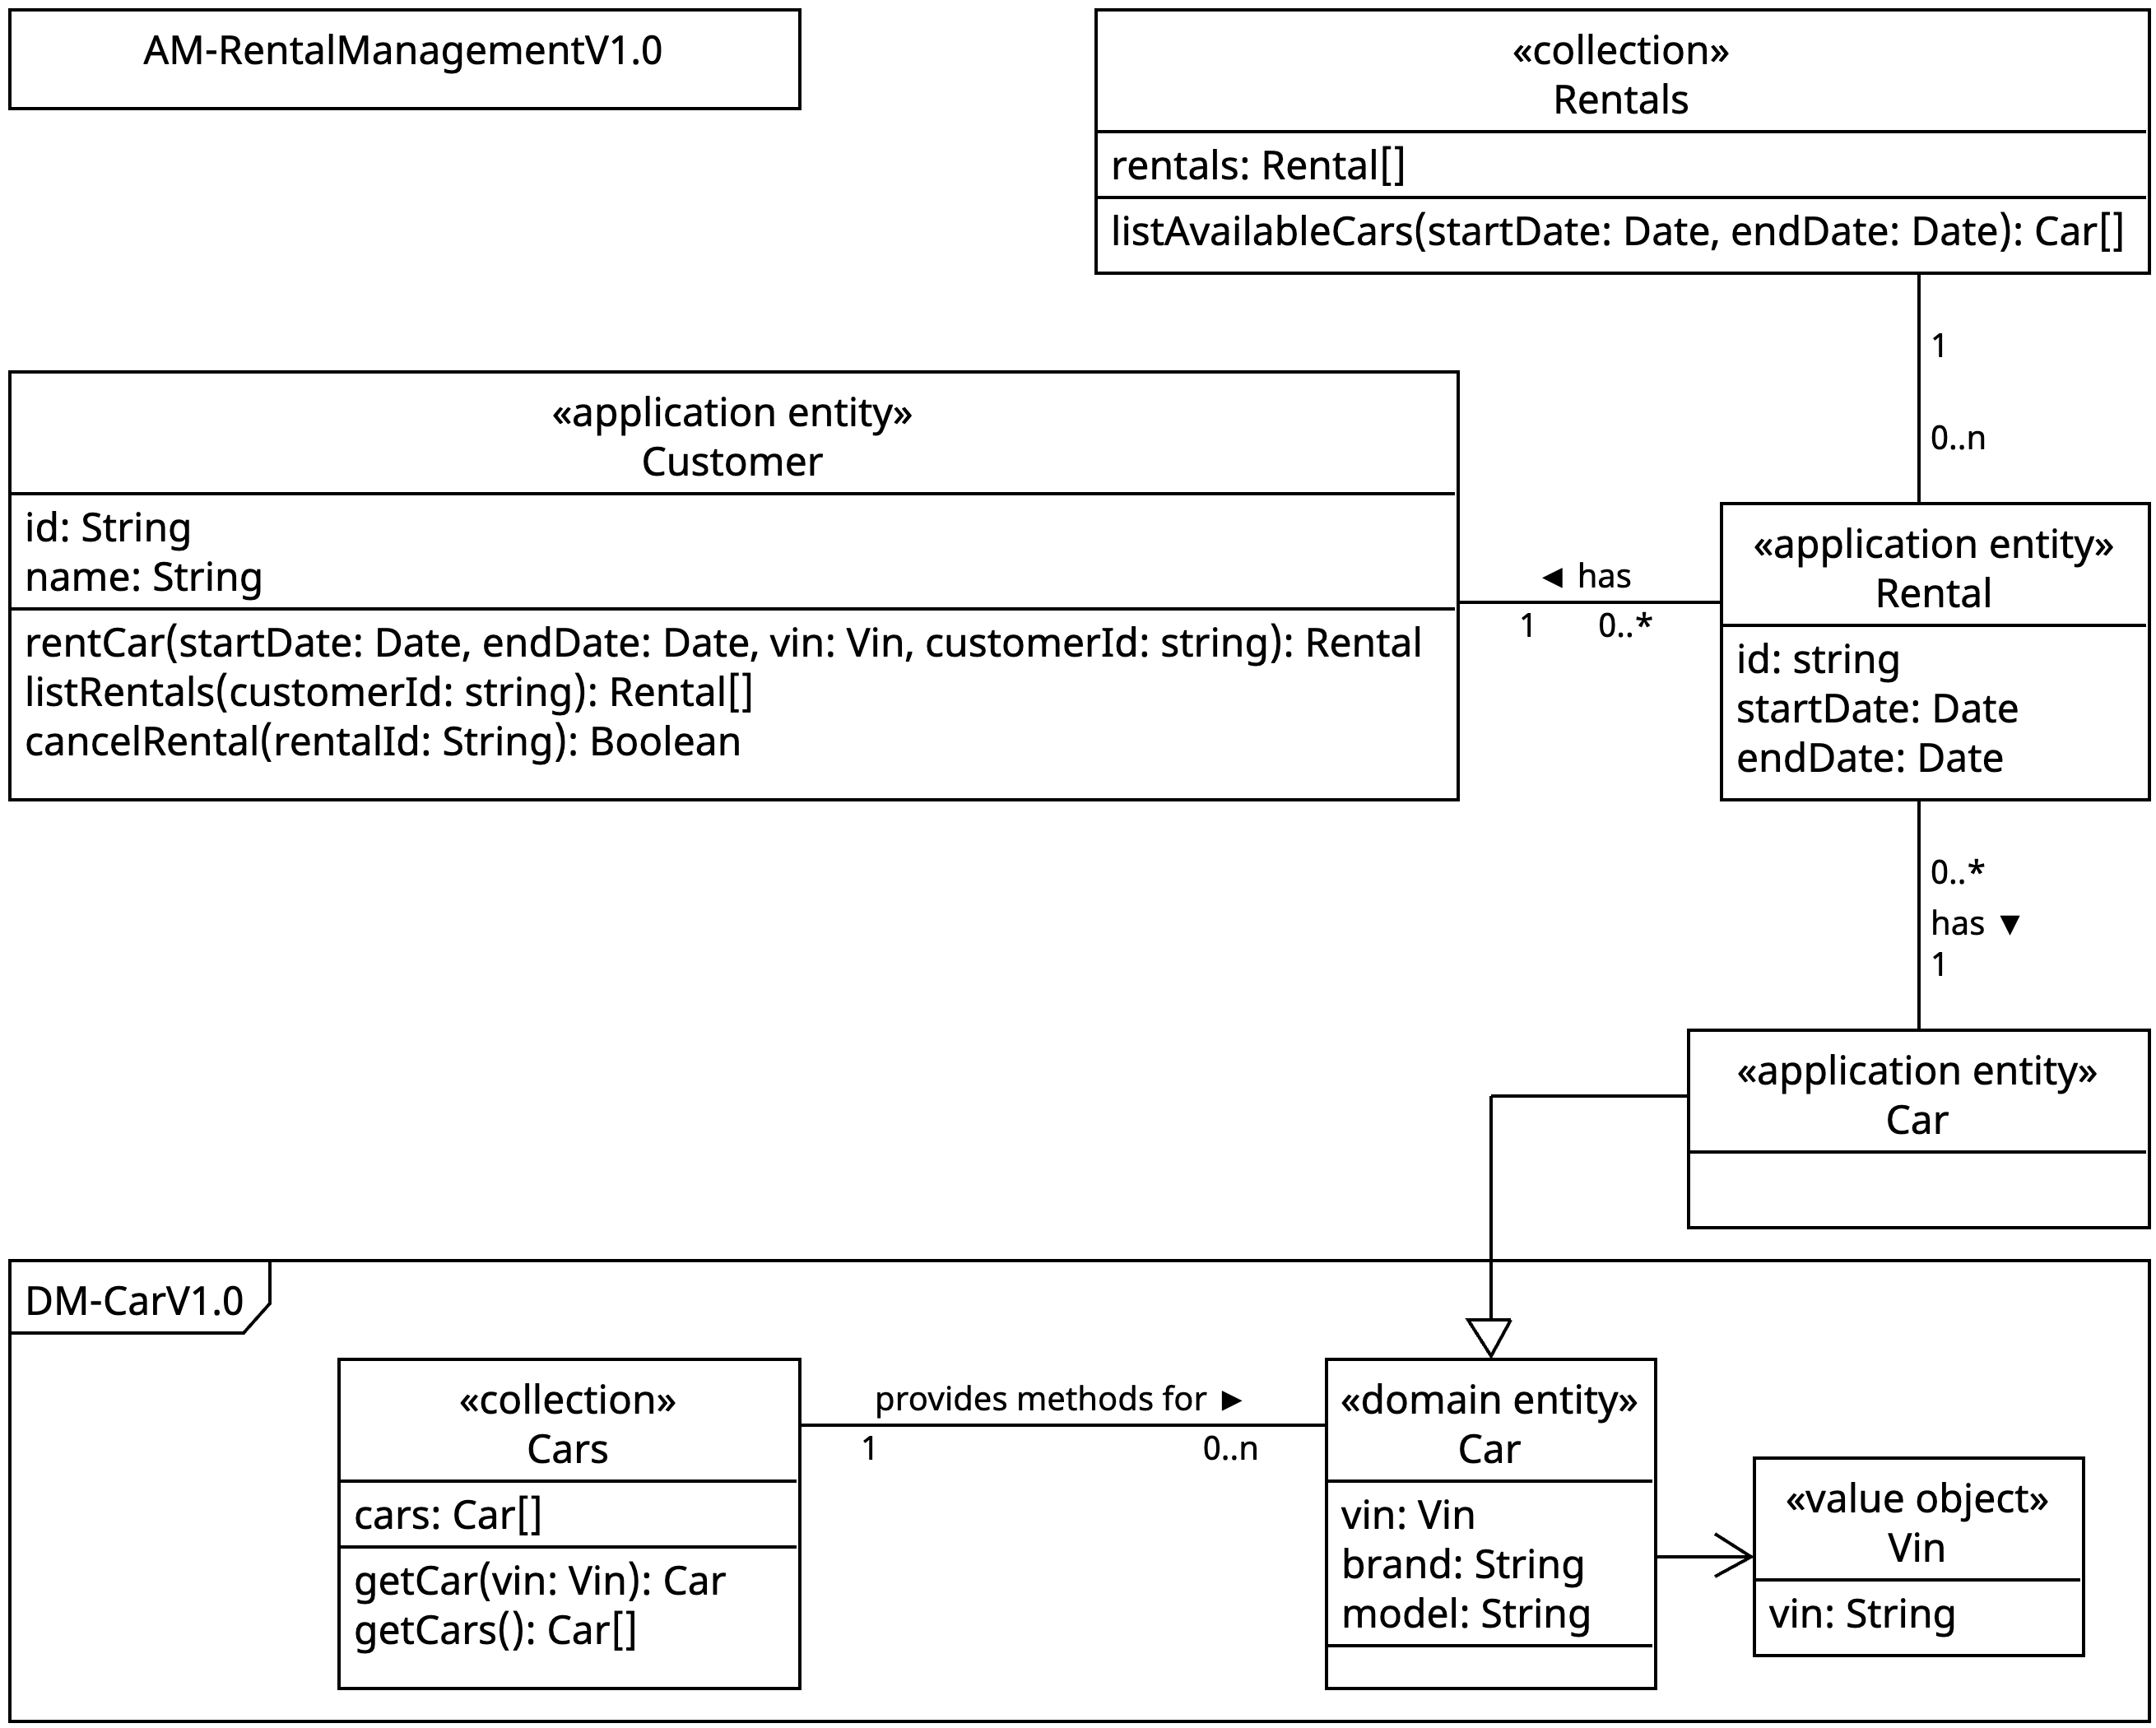
\includegraphics[width=0.8\textwidth]{figures/microservices/rentalManagement/ms_rentalManagement_apiDiagram.png}
    \caption{API Diagram of \texttt{AM-RentalManagementV1.0}}
    \label{fig:ad_am-rental_management_v1.0}
\end{figure}

\subsubsection*{Versioning of the API Diagram}
The version numbers are created using C\&M's versioning as specified in \cite{CM-G-Ver}.
% Explanation of the versioning concept for API diagrams
The initial version of an AM-API diagram is \texttt{1.0}.
The version of an AM API is specified for the first time when the diagram is initially created and reviewed.
It is important to keep the same version for specification and implementation.
The version number is increased when changes occur in the AM-API diagram.
% Explain version numbers of AM-RM and the included DM-Car
Since \texttt{RentalManagementV1.0} and \texttt{DM-CarV1.0} are the initial versions of each microservice, both chosen versions are \texttt{1.0}.

% Which part (X.Y) of the version number is increased when a method RegisterCustomer() is added => what's the new version number
This task assumes a version number to be structured as \texttt{(X.Y)}.
According to the mentioned versioning concept, \texttt{Y} changes when a new function is added to the AM-API diagram.
Therefore, after adding the function \texttt{RegisterCustomer} to the AM-API diagram, the version number is \texttt{1.1}.

\subsubsection*{Relationship between Rental and Car}

\subsubsection*{Relation of Entities Car}

\subsubsection*{API Style}